\section{Potência em C.A.}

\frame{
	\frametitle{Introdução}
	\begin{block}{Classificação}
		A potência pode ser classificada de acordo com o tipo de alimentação que a respectiva carga possui: Potência Elétrica em corrente contínua e em \textbf{corrente alternada}.
	\end{block}
}

\frame{
	\frametitle{Potência em C.A.}
	\begin{block}{Definição}
		\begin{itemize}
			\item Quando se trata de circuitos de C.A. com cargas indutivas e/ou capacitivas, ocorre uma defasagem entre tensão e corrente. Isso nos leva a considerar três tipos de potência:
			      \begin{enumerate}
				      \item\normalsize Potência Ativa ($P$)
				      \item\normalsize Potência Reativa ($Q$)
				      \item\normalsize Potência Aparente ($S$)
			      \end{enumerate}
		\end{itemize}
	\end{block}
}

\frame{
	\frametitle{Conceitos básicos}
	\begin{block}{Por que três tipos de potência?}
		\begin{itemize}
			\item A maioria das cargas das unidades consumidoras consome energia reativa indutiva, tais como: motores, transformadores, reatores para lâmpadas de descarga, fornos de indução, entre outros. As cargas indutivas necessitam de campo eletromagnético para seu funcionamento.
		\end{itemize}
	\end{block}
	\centerline{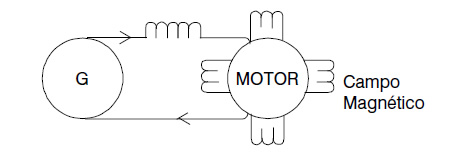
\includegraphics[width=0.8\linewidth]{Figuras/Ch16/campo.jpg}}
}

\frame{
	\frametitle{Potência Ativa ($P$)}
	\begin{block}{Definição}
		\begin{itemize}
			\item Potência que efetivamente realiza \textbf{trabalho} gerando calor, luz, movimento, etc. É medida em \si{\kilo\watt}.
			\item Também chamada de potência \textbf{Real}, é a potência que realmente produz o trabalho na carga.
		\end{itemize}
	\end{block}
}

\frame{
	\frametitle{Potência Reativa ($Q$)}
	\begin{block}{Definição}
		\begin{itemize}
			\item Potência usada apenas para criar e \textbf{manter os campos eletromagnéticos} das cargas indutivas. É medida em \si{\kvar}.
			\item Ela, por sua vez, não realiza o trabalho em si. Isso significa que não é essa energia que liga os eletroeletrônicos e outros equipamentos elétricos, mas ela funciona entre o gerador de energia e a carga em si, sendo responsável por manter o campo eletromagnético ativo em motores, reatores, transformadores, lâmpadas fluorescentes, etc.
		\end{itemize}
	\end{block}
}

\frame{
	\frametitle{Potência Aparente ($S$)}
	\begin{block}{Definição}
		\begin{itemize}
			\item A \textbf{soma entre potência ativa e reativa} gera a potência aparente, medida em \si{\kva}. É esta medida que pode indicar se a energia consumida é o suficiente para um ou outro abastecimento elétrico, assim como apontar onde há a necessidade de melhoria no fornecimento.
		\end{itemize}
	\end{block}
}

\frame{
	\frametitle{Em resumo}
	\begin{block}{Resumindo...}
		\begin{itemize}
			\item A Potência Ativa é a potência que realmente realiza trabalho no sistema.
			\item A Potência Reativa é a potência desperdiçada  pelo sistema.
			\item A Potência Aparente é a Potência total que o sistema retira da rede de alimentação.
		\end{itemize}
	\end{block}
}

\frame{
	\frametitle{Em resumo}
	\centerline{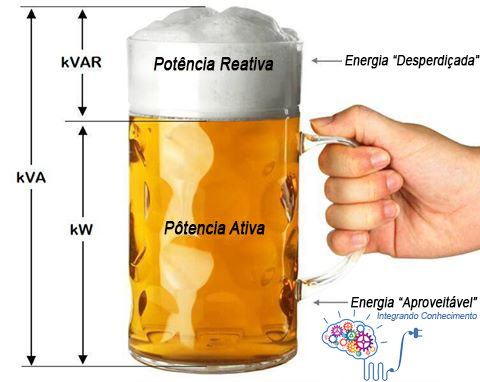
\includegraphics[width=0.8\linewidth]{Figuras/Ch16/chopp.jpg}}
}

\frame{
	\frametitle{Fator de potência}
	\begin{block}{Conceito}
		\begin{itemize}
			\item É a razão entre a potência ativa e a potência aparente.
			\item Ele indica a eficiência do uso da energia.
			\item Um alto fator de potência indica uma eficiência alta e inversamente, um fator de potência baixo indica baixa eficiência energética.
		\end{itemize}
	\end{block}
}

\frame{
	\frametitle{Triângulo de potências}
	\setmyunit{4cm}
	\centering
	\begin{tikzpicture}
		\draw[-Latex] (0,0) -- node[above,rotate=26.5] {Potência aparente (\si{\kva})} (1,0.5);
		\draw[-Latex] (0,0) -- node[below] {Potência ativa (\si{\kilo\watt})} (1,0);
		\draw[-Latex] (1,0) -- node[right] {Potência reativa (\si{\kvar})} (1,0.5);
		
		\coordinate (A) at (1,0);
		\coordinate (O) at (0,0);
		\coordinate (B) at (1,0.5);
		
		\pic[draw, angle radius=25pt,angle eccentricity=1,"$ \phi $" {xshift=4pt,yshift=1pt}] {angle=A--O--B};
	\end{tikzpicture}
	
%	\centerline{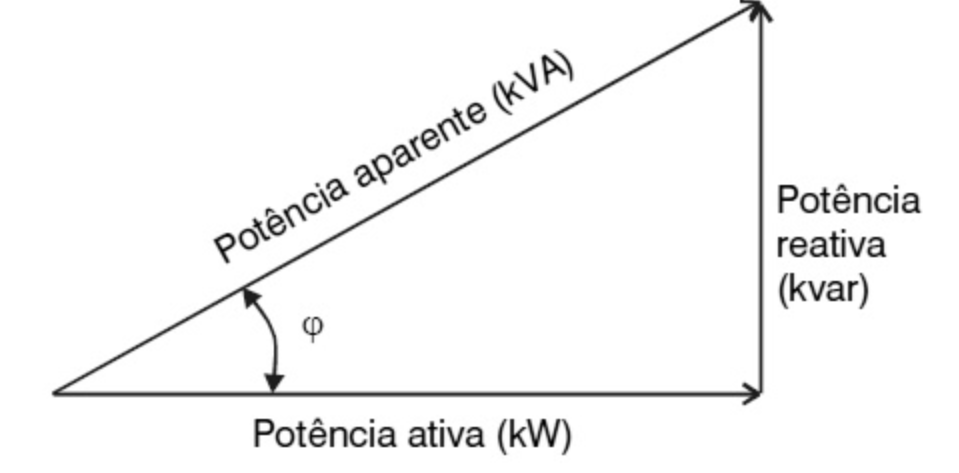
\includegraphics[width=0.8\linewidth]{Figuras/Ch16/triangulo.PNG}}
	\begin{block}{}
		$$\text{FP} = \dfrac{\text{kW}}{\text{KVA}} = \cos \varphi$$ \\
		$$S = U \times I \qquad P = S \cos \varphi \qquad Q = S \sen \varphi$$
	\end{block}
}

\frame{
	\frametitle{Fator de potência}
	\begin{block}{Contextualização}
		\begin{itemize}
			\item O fator de potência mostra se a empresa consome energia elétrica adequadamente ou não.
			\item A legislação (Resolução ANEEL 456/2000) determina que o Fator de Potência deve ser mantido o mais próximo possível da
			      unidade (1), mas permite um \textbf{valor mínimo de \num{0,92}}.
			\item Se o Fator de Potência estiver abaixo desse mínimo, a conta de energia elétrica sofrerá um ajuste em reais.
		\end{itemize}
	\end{block}
}

\frame{
	\frametitle{Fator de potência}
	\begin{block}{O que causa um baixo fator de potência?}
		\begin{itemize}
			\item Motores trabalhando em vazio (sem carga).
			\item Fornos de indução ou arco.
			\item Reatores com baixos fatores de potência no sistema de iluminação.
			\item Máquinas de solda.
			\item Máquinas de tratamento térmico.
			\item Instalação de lâmpadas de descarga (fluorescentes, de vapor de mercúrio e de vapor de sódio).
		\end{itemize}
	\end{block}
}

\frame{
	\frametitle{Fator de potência}
	\begin{block}{Como corrigir o fator de potência?}
		\begin{itemize}
			\item A forma de compensar o baixo Fator de Potência é a instalação de \textbf{bancos de capacitores} em paralelo na entrada de energia ou no próprio equipamento com carga indutiva.
			\item Esses bancos introduzem na instalação uma carga capacitiva, que tem o \textbf{efeito contrário da carga indutiva}.
			\item Isso compensa o baixo Fator de Potência e ajusta o valor para mais próximo de 1, evitando as multas.
		\end{itemize}
	\end{block}
}

\frame{
	\frametitle{Correção do Fator de potência}
	\centerline{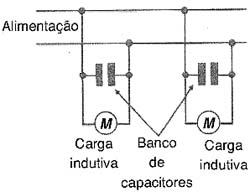
\includegraphics[width=0.6\linewidth]{Figuras/Ch16/banco1.jpg}}
}

\frame{
	\frametitle{Correção do Fator de potência}
	\centerline{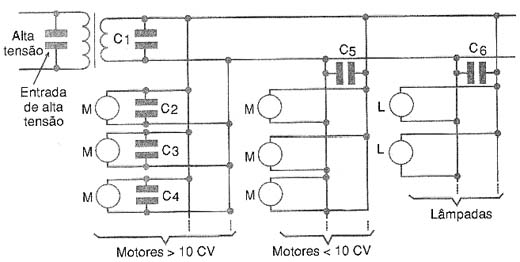
\includegraphics[width=0.7\linewidth]{Figuras/Ch16/banco2.jpg}}
	\begin{block}{Banco de capacitores}
		\begin{itemize}
			\item \textbf{Na entrada de alta tensão}: neste caso, a correção é do fator de potência visto pela concessionária apenas. Internamente, os problemas causados por um baixo fator de potência permanecem.
		\end{itemize}
	\end{block}
}

\frame{
	\frametitle{Correção do Fator de potência}
	\centerline{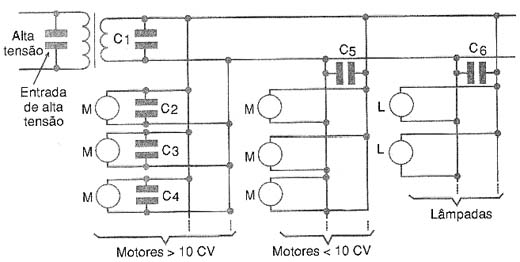
\includegraphics[width=0.7\linewidth]{Figuras/Ch16/banco2.jpg}}
	\begin{block}{Banco de capacitores}
		\begin{itemize}
			\item \textbf{Correção na entrada de baixa tensão}: neste caso, temos uma correção melhor, sendo usados normalmente bancos automáticos de capacitores. Esse tipo de correção é indicado para instalações que possuam muitas cargas com potências e regimes de utilização diferentes.
		\end{itemize}
	\end{block}
}

\frame{
	\frametitle{Correção do Fator de potência}
	\centerline{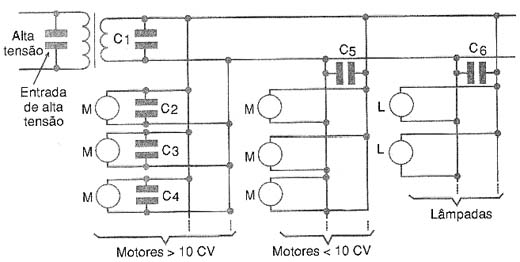
\includegraphics[width=0.7\linewidth]{Figuras/Ch16/banco2.jpg}}
	\begin{block}{Banco de capacitores}
		\begin{itemize}
			\item \textbf{Correção por grupos de cargas}: trata-se de um sistema em que o banco de capacitores é instalado de modo a corrigir setores de uma instalação, normalmente máquinas de potências inferiores a 10 CV. Os capacitores são instalados junto aos quadro de distribuição que alimenta esse equipamentos. A desvantagem é que a corrente não é reduzida na alimentação de cada equipamento.
		\end{itemize}
	\end{block}
}

\frame{
	\frametitle{Correção do Fator de potência}
	\centerline{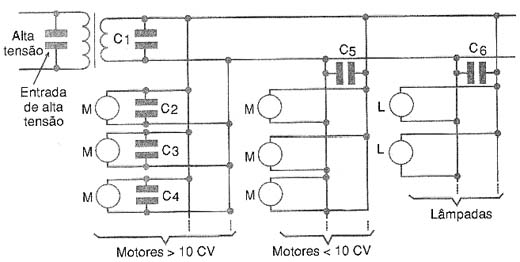
\includegraphics[width=0.7\linewidth]{Figuras/Ch16/banco2.jpg}}
	\begin{block}{Banco de capacitores}
		\begin{itemize}
			\item \textbf{Correção localizada ou individual}: essa correção é feita com a instalação dos capacitores junto a cada equipamento que se pretende corrigir o fator de potência. Tecnicamente é a melhor solução, pois os valores dos capacitores são adequados a cada equipamento.
		\end{itemize}
	\end{block}
}

\frame{
	\frametitle{Correção do Fator de potência}
	\begin{block}{Determinando o valor da capacitância individual}
		$$C = \dfrac{Q}{\omega V^2}$$
	\end{block}
}

\section*{Exercícios}

\frame{
	\frametitle{Exercícios}
	\begin{block}{}
		01.  Uma carga indutiva monofásica consome \SI{10}{\mega\watt} com um fator de potencia em atraso de \num{0.6}. Desenho o triângulo de potência e determine a potência reativa de um capacitor ligado em paralelo com a carga para elevar o fator de potência para \num{0.85}.
	\end{block}
}


\section*{Referências}

\frame{
	\frametitle{Referências e Exercícios Complementares}
	\begin{itemize}
		\item ALEXANDRE, Charles K.; SADIKU, Matthew N. O. Fundamentos de Circuitos Elétricos. 5. ed. Porto Alegre: AMGH, 2013.
	\end{itemize}
	%\centering{\alert{Página 36 - \textbf{1.6.1 até 1.6.5, 1.6.17 até 1.6.19}}} \\
	\centering{\alert{Lista de exercícios 16}}
}